Dans les sections précédentes, nous avons présenté des circuits logiques dits ``combinatoires''. La sortie de ces circuits combinatoires à un instant $t$ dépends uniquement de ses entrées à ce même instant, il n'y a pas de dépendance à l'historique de la valeur des entrées\footnote{modulo les temps de propagation des signaux dans le circuit.}. Nous sommes à deux doigts de construire notre premier microprocesseur mais il nous manque encore un ingrédient. Imaginez, votre amie suzette est ornitologue, elle aimerait bien disposer d'un appareil électronique pour compter les oiseaux lors des migrations et si possible un appareil simple, par exemple avec deux boutons : un bouton pour réinitialiser le compteur et un bouton pour l'incrémenter d'une unité. Vous vous dites ``Super, je sais réaliser un additionneur, mettre une sortie à 0, c'est partie, j'écris la table de vérité''. Et là, vous êtes coincés, parce que pour une configuration d'entrée, par exemple ``bouton incrémenter pressé'', vous avez plusieurs sorties possibles : si il y avait 1 oiseau, il y en a désormais 2, mais si il y avait 2 oiseaux, il y en a désormais 3. Il vous faudrait disposer d'un moyen de représenter un \textbf{état} $n_o$ et qu'à l'appui sur le bouton vous puissiez \textbf{transiter} vers \textbf{l'état} $n_o + 1$. Dis dans l'autre sens, l'état courant dépends de l'entrée et également de l'état précédent. Cette idée est illustrée sur le schéma \ref{fig:intro_seq}. Il nous manque donc la brique permettant de mémoriser un état et c'est le sujet de cette partie.


\begin{figure}[htbp]
\centering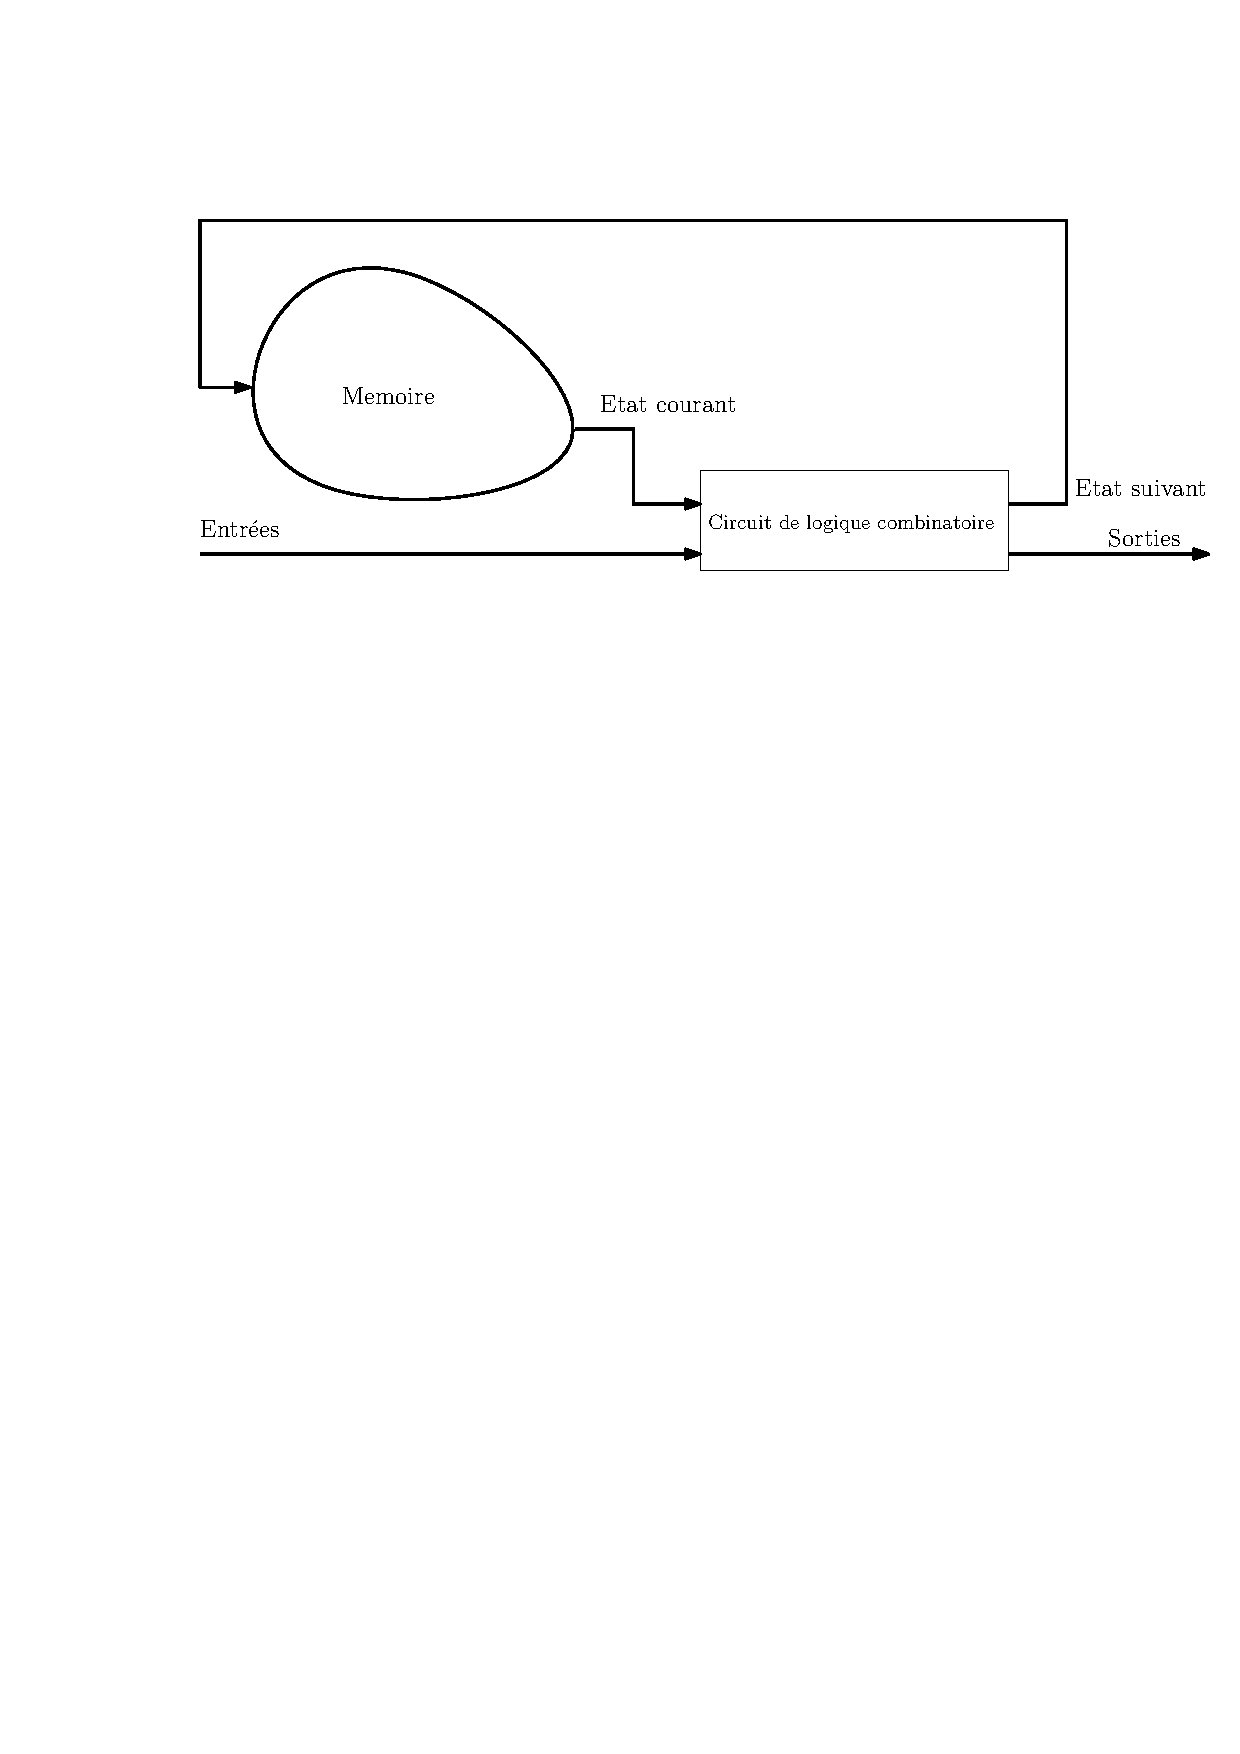
\includegraphics[width=0.75\linewidth]{Figs/intro_seq.pdf}
\caption{\label{fig:intro_seq} Schéma de principe de n'importe quel système numérique. Etant donné un état courant et des entrées, on peut calculer des sorties et le prochain état qu'il suffit de mémoriser pour disposer d'un système dont l'influence des entrées dépends de l'état courant.}
\end{figure}



%\todo{Mentionner l'exemple de la mémoire mais peut être aussi d'un compteur}\\
%\todo{Le verrou D (D latch) peut se voir comme un mutiplexeur à 2 entrées dont l'une est sa sortie, l'autre est la donnée à mémoriser}\\

%% \subsection{Logique séquentielle synchrone et asynchrone}

%% Le verrou (\emph{latch}) est asynchrone (pas de signal d'horloge); la bascule (\emph{flip-flop}) est synchrone (avec un signal d'horloge). 

\subsection{Verrou/Bascule RS}

Le verrou RS (\emph{Reset}/\emph{Set}) possède deux entrées ($S$, $R$) et deux sorties ($Q,\bar{Q}$) comme illustré sur la figure \ref{fig:verrou_rs}. Le circuit contient des boucles de rétroaction et sa sortie est dépendante de l'historique de ses entrées comme nous allons le voir.

\begin{figure}[htbp]
\begin{center}
\tikzstyle{branch}=[fill,shape=circle,minimum size=3pt,inner sep=0pt]
\begin{tikzpicture}[label distance=2mm]

    \node[nor gate US, draw, logic gate inputs=nn] at (0,0) (Nor1) {};
    \node[nor gate US, draw, logic gate inputs=nn] at (0,-2) (Nor2) {};

    \node (S) at ($(Nor1.input 1) - (1,0)$) {$Set$};
    \node (R) at ($(Nor2.input 2) - (1,0)$) {$Reset$};
    \node (bQ) at ($(Nor1.output) + (1, 0)$) {$\bar{Q}$};
    \node (Q) at ($(Nor2.output) + (1, 0)$) {$Q$};

    \node at ($(Nor1.output) - (0.5,0)$) {$1$};
    \node at ($(Nor2.output) - (0.5,0)$) {$2$};

    \draw (S) -- (Nor1.input 1);
    \draw (Nor2.output) -- ([xshift=0.5cm]Nor2.output) -- ++(0, 0.5) -- ([xshift=-0.5cm,yshift=-0.5cm]Nor1.input 2) -- ([xshift=-0.5cm]Nor1.input 2) -- (Nor1.input 2);
    \draw (Nor1.output) -- (bQ);

    \draw (R) -- (Nor2.input 2);
    \draw (Nor1.output) -- ([xshift=0.5cm]Nor1.output) -- ++(0, -0.5) -- ([xshift=-0.5cm,yshift=+0.5cm]Nor2.input 1) -- ([xshift=-0.5cm]Nor2.input 1) -- (Nor2.input 1);
    \draw (Nor2.output) -- (Q);
\end{tikzpicture}
\end{center}
\caption{\label{fig:verrou_rs} Un verrou RS (Reset/Set) formé par deux portes NOR (les numéros dans les portes facilitent l'explication du fonctionnement du circuit) avec des connections réentrantes.}
\end{figure}

Étudions le comportement du verrou pour les entrées $(0,0)$, $(0,1)$, et $(1,0)$, on verra un peu plus loin que l'entrée $(1,1)$ conduit à un état instable et qu'on s'interdira donc cette entrée. La figure~\ref{fig:chrono_rs_1} présente l'évolution au cours du temps des entrées et des sorties du verrou. A l'instant $t_0$, l'entrée passe de $(R,S) = (0,0)$ à $(R,S) = (0,1)$. Il existe une période transitoire entre $t_0$ et $t_0 + \Delta$ avant que le circuit n'atteigne un état stable. En effet, à $t_0$, lorsque $S$ passe à $1$, seules les entrées de la première porte NOR changent. Ses entrées étant $(S, Q) = (1,0)$, la sortie passe à $\bar{Q} = 0$. Cela affecte alors à $t_0 + \Delta/2$ la deuxième porte NOR qui, ayant ses entrées à $(\bar{Q}, R) = (0,0)$ voit sa sortie passer à $Q = 1$ après un délai de $\Delta /2$. Au temps $t_0+\Delta$, les sorties du verrou sont alors à $(Q,\bar{Q}) = (1, 0)$ qui est un état stable pour le circuit. Le délai $\Delta/2$ corresponds au temps de propagation des signaux dans les portes logiques NOR et est de l'ordre de quelques dizaines à centaines de nanosecondes\footnote{Voir par exemple la notice technique de la puce 74HC02 ou CD4001}. \\

\begin{figure}[htbp]
\begin{center}
\begin{tikztimingtable}[
    timing/coldist=2pt,     % column distance
    xscale=1,yscale=1, % scale diagrams
    semithick               % set line width
]
$R$       & 2L       LLLLLL       LLLLLL       HHHHHH       LLLLLL  \\
$S$       & 2L       HHHHHH       LLLLLL       LLLLLL       LLLLLL  \\
$Q$       & 2L       LLHHHH       HHHHHH       HLLLLL       LLLLLL\\
$\bar{Q}$ & 2H N(Q1) HLLLLL N(Q2) LLLLLL N(Q3) LLHHHH N(Q4) HHHHHH \\
          & SS       SSSSSS       SSSSSS       SSSSSS       SSSSSS\\
\extracode
  %\tablerules
  %\tablegrid
  \begin{pgfonlayer}{background}
    \vertlines[help  lines]{2,4,8,14,16,20}
    \draw[thick,<->,shorten >=2pt,shorten <=2pt,>=stealth] (2, -8) -- (4,-8);
    \draw [anchor=mid] node at (3,-7) {\tiny $\Delta$};
    \draw [anchor=north] let \p1=(Q1) in node at (\x1,-9) {$t_0$};

    \draw [anchor=north] let \p1=(Q2) in node at (\x1,-9) {$t_1$};

    \draw[thick,<->,shorten >=2pt,shorten <=2pt,>=stealth] (14, -8) -- (16,-8);
    \draw [anchor=mid] node at (15,-7) {\tiny $\Delta$};
    \draw [anchor=north] let \p1=(Q3) in node at (\x1,-9) {$t_2$};

    \draw [anchor=north] let \p1=(Q4) in node at (\x1,-9) {$t_3$};
  \end{pgfonlayer}
\end{tikztimingtable}
\end{center}
\caption{\label{fig:chrono_rs_1} Chronogramme d'un verrou RS.}
\end{figure}

A l'instant $t_1$, les entrées repassent à $(R,S) = (0,0)$. Les entrées de la première porte NOR étant $(S, Q) = (0, 1)$, la sortie reste à $\bar{Q} = 0$. Pour la deuxième porte, il en est de même; ses entrées étant $(\bar{Q}, R) = (0, 0)$, sa sortie reste à $\bar{Q} = 1$. Cet état est un état de mémorisation, le verrou reste dans l'état dans lequel il était. \\

Passons maintenant, à l'instant $t_3$, les entrées à $(R,S) = (1,0)$. Seule la deuxième porte NOR voit ses entrées changer pour le moment et passer à $(\bar{Q}, R) = (0, 1)$, sa sortie passe donc à $Q = 0$. Cela a pour conséquence d'affecter la première porte; ayant les entrées $(S, Q) = (0, 0)$, sa sortie passe à $\bar{Q} = 1$. Cet état est un état stable. \\

 La table de vérité du verrou $RS$ est donnée ci-dessous~:\\
\begin{center}
\begin{tabular}{cc||ccl}
$R$ & $S$ & $Q$ & $\bar{Q}$ & Remarque\\
\hline
0 & 0 & $x$ & $\bar{x}$ & Maintien de l'état précédent\\
0 & 1 & 1 & 0 & Mise à un\\
1 & 0 & 0 & 1 & Mise à zéro\\
1 & 1 & 0 & 0 & Etat interdit 
\end{tabular}
\end{center}

\begin{framed}
\textbf{Résumé : } Un verrou RS ne s'utilise que pour les entrées $(R,S) \in \{(0,0), (0,1), (1,0)\}$.
\begin{itemize}
\item l'entrée $R=0$, $S=1$ met à 1 la sortie du verrou $Q = 1$, $\bar{Q}=0$,
\item l'entrée $R=1$, $S=0$ met à 0 la sortie du verrou $Q = 0$, $\bar{Q}=1$,
\item l'entrée $R=0$, $S=0$ laisse la sortie du verrou dans son état
\end{itemize}
\end{framed}

% 
% http://www.iitg.ernet.in/asahu/cs221/Lects/Lec13.pdf
Si les entrées $R$ et $S$ sont simultanément à un niveau haut, le système entre dans un état pour lequel les sorties $Q$ et $\bar{Q}$ ne sont pas complémentaires et est considéré comme un état interdit. En effet, le verrou peut alors entrer dans un régime instable. Si les entrées $R$ et $S$ repassent simultanément à un niveau bas $(R, S) = (0,0)$ alors que les sorties étaient également à l'état bas $(Q, \bar{Q}) = (0,0)$, dans le cas d'un circuit tout à fait symétrique, les sorties vont passer à $(1,1)$ puis $(0,0)$, ... En pratique, le circuit n'est pas parfaitement symétrique parce que les portes (et leur délais de propagation) ne sont pas tout à fait identiques et les connexions entre les sorties et les entrées non plus. Cette asymétrie conduira alors le verrou à atteindre un état stable mais en un temps arbitrairement long et il finira dans un état impossible à prédire. C'est la raison pour laquelle l'entrée $(R,S) = (1,1)$ est interdite.\\


\paragraph{Exemple : mémoriser l'appui d'un bouton:\\}

Pour illustrer l'effet mémoire d'un verrou RS, considérons deux circuits représentés sur les figures \ref{fig:ill_verrou}a et \ref{fig:ill_verrou}b. Sur la figure \ref{fig:ill_verrou}a, nous avons simplement un interrupteur qui contrôle l'allumage d'une lumière. Si on appuis sur le bouton, la lumière s'allume mais dés qu'on relâche le bouton, la lumière s'éteint. Si on modifie un peu le circuit pour placer un verrous R/S qu'on peut contrôler avec deux boutons ``allume'' et ``éteint'', on peut maintenir la lumière allumée même lorsque le bouton ``allume'' est relâché. On a donc bien mémorisé l'état ``allumé''. 

\begin{figure}[htbp]
\begin{tabular}{cc}
\begin{circuitikz}
\draw[color=black, thick]
    (0,0) to [push button,l=allume] (1.5, 0) to [lamp] (3.0, 0) to [R] (4.5, 0) to (5, 0) node[ground] {}
    (0,0) to [short,-o](0, 2) node[right]{$V^+$};
\end{circuitikz}&
\begin{circuitikz}[scale=0.9,transform shape]
\draw[color=black, thick]
    (4,0.1) node[nor gate US, draw, logic gate inputs=nn] (Nor2) {}
    (4,2.1) node[nor gate US, draw, logic gate inputs=nn] (Nor1) {}
    (0,0) to [push button,l=éteint] (2, 0) to (Nor2.input 2)
    (0,2.2) to [push button,l=allume] (2, 2.2) to (Nor1.input 1)  
    (Nor2.output) to [R] ([xshift=2.5cm]Nor2.output) to [lamp] ([xshift=3.5cm]Nor2.output) to ([xshift=4cm]Nor2.output) node[ground]{}
    (0,0) to [short,-o](0,3) node[above]{$V^+$}
    (Nor1.output) to ([xshift=.5cm]Nor1.output) node(Nor1o) {} to ([yshift=-0.5cm]Nor1o) to ([xshift=-.5cm,yshift=.5cm]Nor2.input 1) to ([xshift=-.5cm]Nor2.input 1) to (Nor2.input 1)
    (Nor2.output) to ([xshift=.5cm]Nor2.output) node(Nor2o) {} to ([yshift=0.5cm]Nor2o) to ([xshift=-.5cm,yshift=-.5cm]Nor1.input 2) to ([xshift=-.5cm]Nor1.input 2) to (Nor1.input 2)
    ([xshift=-1cm]Nor1.input 1) to [R, bipoles/length=0.5cm] ([xshift=-1cm,yshift=-1cm]Nor1.input 1) |- ([xshift=-1.5cm,yshift=-1cm]Nor1.input 1) node[ground,rotate=-90](gndpulldown) {}
    ([xshift=-1cm]Nor2.input 2) to [R, bipoles/length=0.5cm] ([xshift=-1cm,yshift=1cm]Nor2.input 2) |- (gndpulldown);
\end{circuitikz}\\
a) & b)
\end{tabular}
\caption{\label{fig:ill_verrou}a) Si le bouton est appuyé, la lumière s'allume; Si le bouton est relâché, la lumière s'éteint. b) Avec un verrou R/S, si on appuis sur le bouton ``allume'', la lumière s'allume et reste allumé même si on relâche le bouton. La lumière s'éteindra en pressant sur le bouton ``éteint''.}
\end{figure}




 L'un des inconvénients du verrou RS est que son état est tout de même très dépendant de ses entrées $R$ et $S$ puisque seul l'état $(R,S) = (0,0)$ est un état de mémoire. Il est souvent préférable d'avoir plus de contrôle sur les instants o{\`u} l'on souhaite mémoriser une donnée (fournie par R et S). On définit alors le verrou RS contrôlé (\emph{gated RS latch}) comme sur la figure~\ref{fig:gated_verrou_rs}. La seule différence avec le verrou RS est l'introduction d'un signal de contrôle qui force les entrées des portes NOR provenant de $R$ et $S$ à un niveau bas lorsque $Enable = 0$. Si $Enable=1$, ce circuit se comporte comme un verrou RS.


\begin{figure}[htbp]
\begin{center}
\tikzstyle{branch}=[fill,shape=circle,minimum size=3pt,inner sep=0pt]
\begin{tikzpicture}[label distance=2mm]

    \node[nor gate US, draw, logic gate inputs=nn] at (0,0) (Nor1) {};
    \node[nor gate US, draw, logic gate inputs=nn] at (0,-2) (Nor2) {};
    \node[and gate US, draw, logic gate inputs=nn] at ($(Nor1.input 1) - (1, 0)$) (And1) {};
    \node[and gate US, draw, logic gate inputs=nn] at ($(Nor2.input 2) - (1, 0)$) (And2) {};

    \node[anchor=east] (S) at ($(And1.input 1) - (1,0)$) {$Set$};
    \node[right] (E) at (-4,-1) {$Enable$};
    \node[anchor=east] (R) at ($(And2.input 2) - (1,0)$) {$Reset$};
    \node (bQ) at ($(Nor1.output) + (1, 0)$) {$\bar{Q}$};
    \node (Q) at ($(Nor2.output) + (1, 0)$) {$Q$};

    \node at ($(Nor1.output) - (0.5,0)$) {};
    \node at ($(Nor2.output) - (0.5,0)$) {};

    \draw (S) -- (And1.input 1);
    \draw (And1.output) -- (Nor1.input 1);
    \draw (R) -- (And2.input 2);
    \draw (And2.output) -- (Nor2.input 2);
    \draw (E) -| ($(And1.input 2)-(0.5,0)$) -- (And1.input 2);
    \draw (E) -| ($(And2.input 1)-(0.5,0)$) -- (And2.input 1);



    \draw (Nor2.output) -- ([xshift=0.5cm]Nor2.output) -- ++(0, 0.5) -- ([xshift=-0.5cm,yshift=-0.5cm]Nor1.input 2) -- ([xshift=-0.5cm]Nor1.input 2) -- (Nor1.input 2);
    \draw (Nor1.output) -- (bQ);

    \draw (Nor1.output) -- ([xshift=0.5cm]Nor1.output) -- ++(0, -0.5) -- ([xshift=-0.5cm,yshift=+0.5cm]Nor2.input 1) -- ([xshift=-0.5cm]Nor2.input 1) -- (Nor2.input 1);
    \draw (Nor2.output) -- (Q);
\end{tikzpicture}
\end{center}
\caption{\label{fig:gated_verrou_rs}Verrou RS contrôlé (\emph{gated RS latch}).}
\end{figure}

Ce verrou fonctionne sur des niveaux du signal de contrôle : lorsque le signal de contrôle \emph{enable} est à l'état haut, on retrouve un verrou RS et lorsque le signal de contrôle \emph{enable} est à l'état bas le verrou est dans un état de mémoire, peu importe ce qui se passe sur ses entrées (cf fig.\ref{fig:chrono_gated_rs_1}).

\begin{figure}[htbp]
\begin{center}
\begin{tikztimingtable}[
    timing/coldist=2pt,     % column distance
    xscale=1,yscale=1, % scale diagrams
    semithick               % set line width
]
$E$       & LH       HHHHHH       HHHLLL       LLLLLL       LLLLLL \\
$R$       & 2L       LLLLLL       LLLLLL       HHHHHH       LLLLLL  \\
$S$       & 2L       HHHHHH       LLLLLL       LLLLLL       LLLLLL  \\
$Q$       & 2L       LLHHHH       HHHHHH       HHHHHH       HHHHHH \\
$\bar{Q}$ & 2H N(Q1) HLLLLL N(Q2) LLLLLL N(Q3) LLLLLL N(Q4) LLLLLL \\
          & SS       SSSSSS       SSSSSS       SSSSSS       SSSSSS\\
\extracode
  %\tablerules
  %\tablegrid
  \begin{pgfonlayer}{background}
    \vertlines[help  lines]{2,4,8,14}
    \draw[thick,<->,shorten >=2pt,shorten <=2pt,>=stealth] (2, -10) -- (4,-10);
    \draw [anchor=mid] node at (3,-9) {\tiny $\Delta$};
    \draw [anchor=north] let \p1=(Q1) in node at (\x1,-10) {$t_0$};

    \draw [anchor=north] let \p1=(Q2) in node at (\x1,-10) {$t_1$};

    \draw [anchor=north] let \p1=(Q3) in node at (\x1,-10) {$t_2$};
  \end{pgfonlayer}
\end{tikztimingtable}
\end{center}
\caption{\label{fig:chrono_gated_rs_1} Chronogramme d'un verrou RS contrôlé.}
\end{figure}



%Le verrou RS (\emph{RS-latch}) est un circuit asynchrone: le changement de la sortie est commandé par le changement des entrées $R$ et $S$. Parfois, on souhaite contrôler 

% A voir sur les bascules D : http://www.eng.auburn.edu/~strouce/class/elec2200/elec2200-9.pdf

%\textbf{Illustration avec une mémoire 2 nor + 2 leds + 2 boutons sous logisim}

\subsection{Verrou D}

Nous sommes presque arrivé à la réalisation d'une mémoire à un bit. On souhaite mémoriser un bit, notons le $D$. Il suffit alors de considérer le verrour RS en connectant convenablement les entrées Set et Reset à $D$ comme sur la figure \ref{fig:verrou_d}

\begin{figure}[htbp]
   \begin{minipage}[c]{.7\linewidth}
\tikzstyle{branch}=[fill,shape=circle,minimum size=3pt,inner sep=0pt]
\begin{tikzpicture}[label distance=2mm]

    \node[nor gate US, draw, logic gate inputs=nn] at (0,0) (Nor1) {};
    \node[nor gate US, draw, logic gate inputs=nn] at (0,-2) (Nor2) {};
    \node[and gate US, draw, logic gate inputs=nn] at ($(Nor1.input 1) - (1, 0)$) (And1) {};
    \node[and gate US, draw, logic gate inputs=nn] at ($(Nor2.input 2) - (1, 0)$) (And2) {};
    \node[not gate US, draw] at ($(And2.input 2) - (1,0)$) (Not) {};

    \node (D) at ($(And1.input 1) - (4,0)$) {$D$};

    \node[right] (E) at (-6,-1) {$Enable$};
    \node (bQ) at ($(Nor1.output) + (1, 0)$) {$\bar{Q}$};
    \node (Q) at ($(Nor2.output) + (1, 0)$) {$Q$};

    \node at ($(Nor1.output) - (0.5,0)$) {};
    \node at ($(Nor2.output) - (0.5,0)$) {};

    \draw (D) -- (And1.input 1) node [midway,circ] (S) {};
    \draw (S) |- (Not.input);

    \draw (And1.output) -- (Nor1.input 1);
    \draw (Not.output) -- (And2.input 2);
    \draw (And2.output) -- (Nor2.input 2);
    \draw (E) -| ($(And1.input 2)-(0.5,0)$) node[midway,circ]{} -- (And1.input 2);
    \draw (E) -| ($(And2.input 1)-(0.5,0)$) -- (And2.input 1);



    \draw (Nor2.output) -- ([xshift=0.5cm]Nor2.output) -- ++(0, 0.5) -- ([xshift=-0.5cm,yshift=-0.5cm]Nor1.input 2) -- ([xshift=-0.5cm]Nor1.input 2) -- (Nor1.input 2);
    \draw (Nor1.output) -- (bQ);

    \draw (Nor1.output) -- ([xshift=0.5cm]Nor1.output) -- ++(0, -0.5) -- ([xshift=-0.5cm,yshift=+0.5cm]Nor2.input 1) -- ([xshift=-0.5cm]Nor2.input 1) -- (Nor2.input 1);
    \draw (Nor2.output) -- (Q);
\end{tikzpicture}\\\centering a)
\end{minipage}\hfill
\begin{minipage}[c]{.1\linewidth}
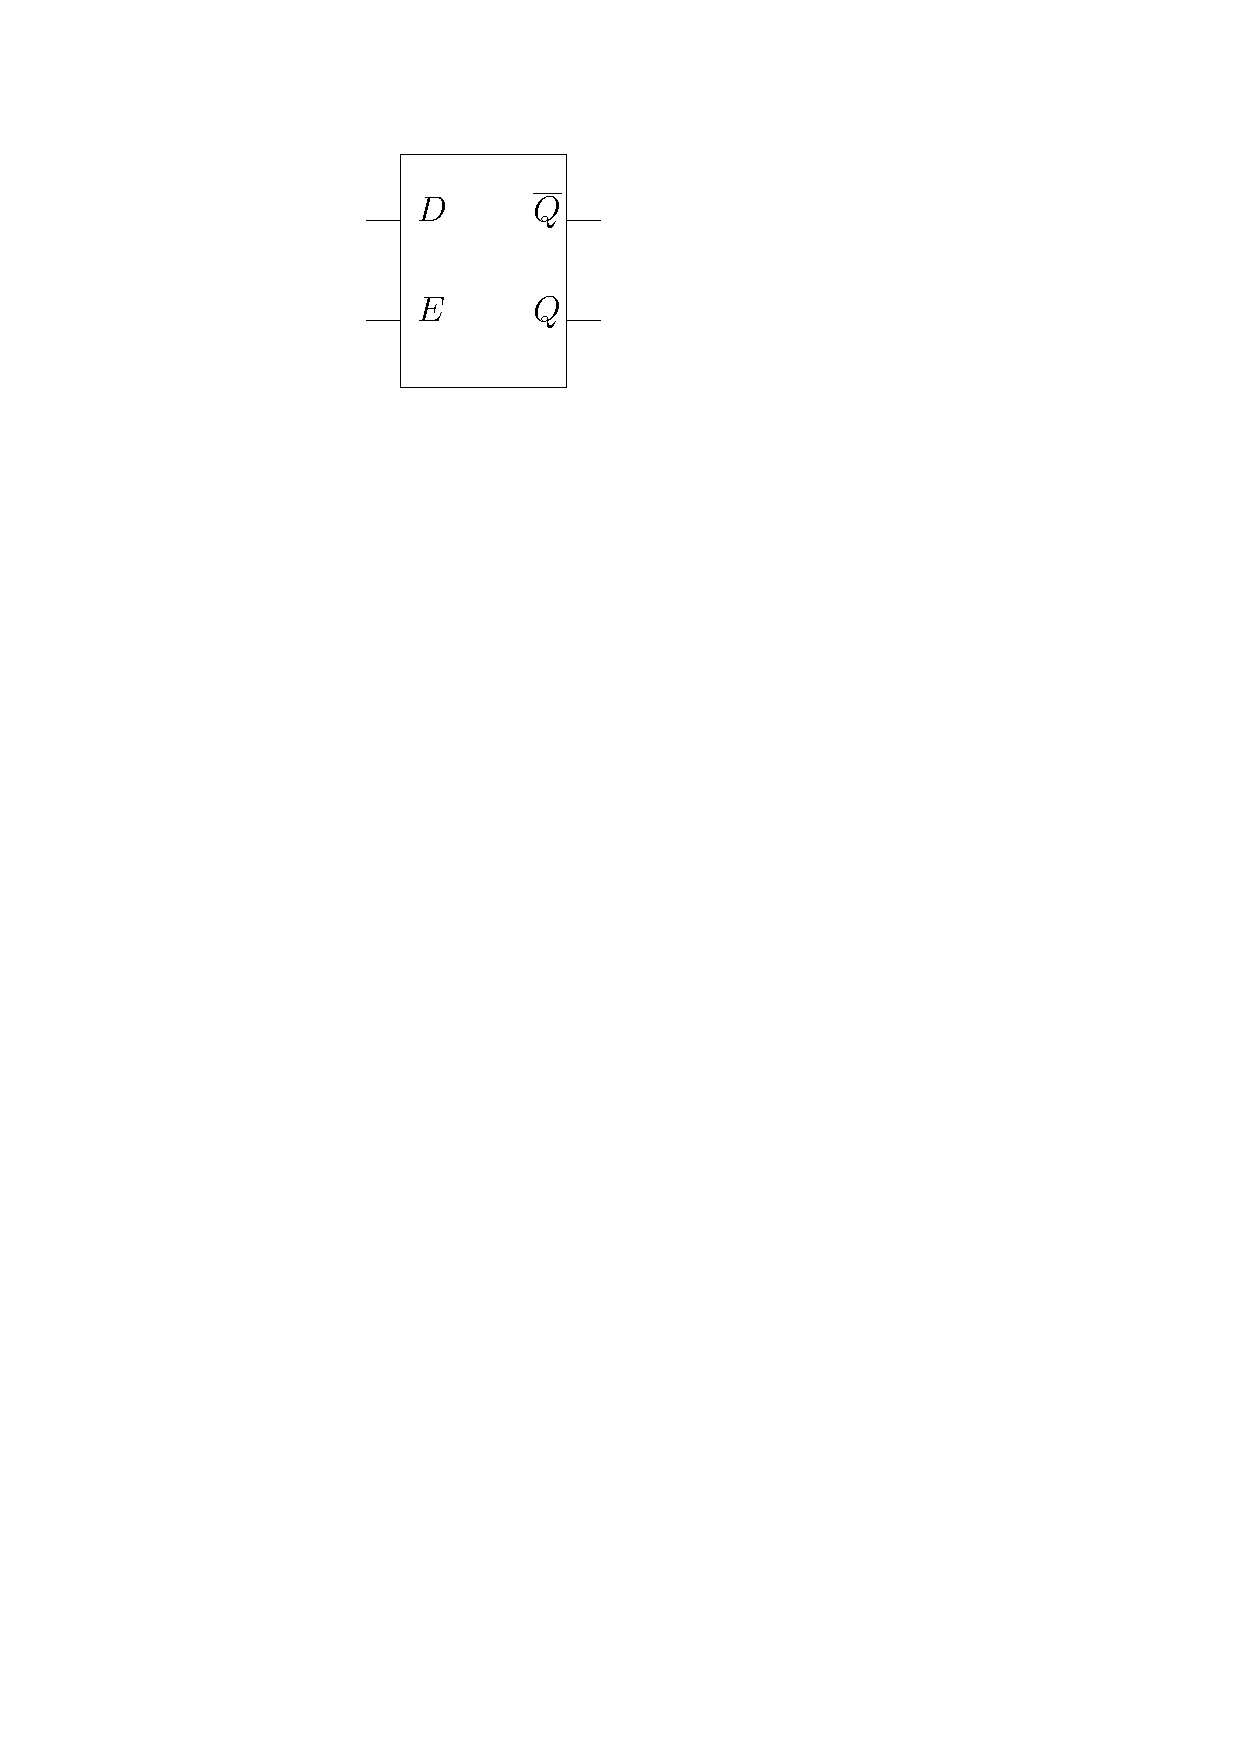
\includegraphics[width=\columnwidth]{Figs/verrou_D.pdf}
\\\centering b)
\end{minipage}
\caption{\label{fig:verrou_d} a) Un verrou D (\emph{Data-latch}) construit à partir d'un verrou RS en connectant les entrées Reset et Set : $Set = D, Reset = \overline{D}$. b) Représentation schématique d'un verrou D.}
\end{figure}

Ce circuit assure aussi que l'état instable du verrou $RS$ obtenu avec les entrées $R=1, S=1$ n'est jamais obtenu puisque les entrées $R$ et $S$ son câblées pour être complémentaires.

\begin{framed}
\textbf{Résumé : } Un verrou D a deux entrées $Date$ et $Enable$ et fonctionne de la manière suivante :
\begin{itemize}
\item si l'entrée $E=1$, alors $Q = D$, on dit que le verrou est transparent,
\item si l'entrée $E=0$, alors le verrou est dans un état mémoire, sa sortie ne changera pas si $D$ change et ne pourra changer que si $E$ passe à l'état haut
\end{itemize}
\end{framed}



\subsection{Systèmes logiques synchrones : horloge et fronts montants}

On précisait en introduction que le but du circuit mémoire que nous cherchons à construire est de mémoriser l'état courant d'un système, peu importe ce que représente cet état. On comprends bien que le verrou D recevra sur l'entrée D l'état mais qu'en est-il de l'entrée Enable ? On va ici considérer que la transition d'un état à un autre est rythmée par une horloge (un signal périodique en créneaux) et cela va nous conduire à construire des \emph{systèmes logiques synchrones}. Lorsque les transitions d'état sont produites par les entrées, sans être dépendantes d'un signal d'horloge, on parle de \emph{systèmes logiques asynchrones} mais nous n'en parlerons pas ici. 

Donc, pour nous, c'est une horloge qui va dicter les instants auxquels un système peut changer d'état. Un signal d'horloge est représenté sur la figure \ref{fig:clk}. Ce signal est périodique de période $T$ et de fréquence $f = 1/T$.

\begin{figure}[htbp]
\begin{center}
\begin{tikztimingtable}[
    timing/coldist=2pt,     % column distance
    xscale=1,yscale=1, % scale diagrams
    semithick               % set line width
]
$Horloge$       & 12{2C} C\\
& \\
\extracode
  %\tablerules
  %\tablegrid
  \begin{pgfonlayer}{background}
    \vertlines[help  lines]{2,6}
    \draw[thick,<->,shorten >=2pt,shorten <=2pt,>=stealth] (2, -3) -- (6,-3);
    \draw [anchor=mid] node at (4,-2) {$T$};
  \end{pgfonlayer}
\end{tikztimingtable}
\end{center}
\caption{\label{fig:clk} Un signal d'horloge est un signal en créneaux, périodique de période $T$ et de fréquence $f = 1/T$.}
\end{figure}

Si on utilise directement ce signal d'horloge comme entrée $Enable$ à un verrou D, le verrou est transparent sur le niveau haut de l'horloge comme illustré sur la figure \ref{fig:chrono_verrou_D}.

\begin{figure}[htbp]
\begin{center}
\begin{tikztimingtable}[
    timing/coldist=2pt,     % column distance
    xscale=1,yscale=2, % scale diagrams
    semithick               % set line width
]
$Horloge$ & 8L 8H 8L 8H \\
$D$       & 2L 3H 2L 2H  1L 2H 1L 1H 1L 3H  6L   2L 3H 3L \\
$Q$       & 8L 1H 1L 2H 1L 1H 1L 9H    2L 3H 3L\\
\extracode
  %\tablerules
  %\tablegrid
\end{tikztimingtable}
\end{center}
\caption{\label{fig:chrono_verrou_D} Chronogramme d'un verrou D contrôlé par une horloge. La sortie du verrou est autorisé à changer (il est transparent) tant que le signal d'horloge est au niveau haut.}
\end{figure}


Pour s'assurer qu'une seule transition ait lieu, il faut garantir que la mise à jour de la mémoire ne se fasse qu'à des instants particuliers, comme par exemple le front montant de l'horloge\footnote{on pourrait aussi considérer le front descendant de l'horloge}, lorsque ce signal passe du niveau bas $0$ au niveau haut $1$ (fig. \ref{fig:clk_fronts}). En chaînant deux verrous D, on construit ce qu'on appelle la bascule D maître escale pour laquelle on est assuré que la mise à jour de la sortie n'a lieu que sur un front d'horloge.

\begin{figure}[htbp]
\centering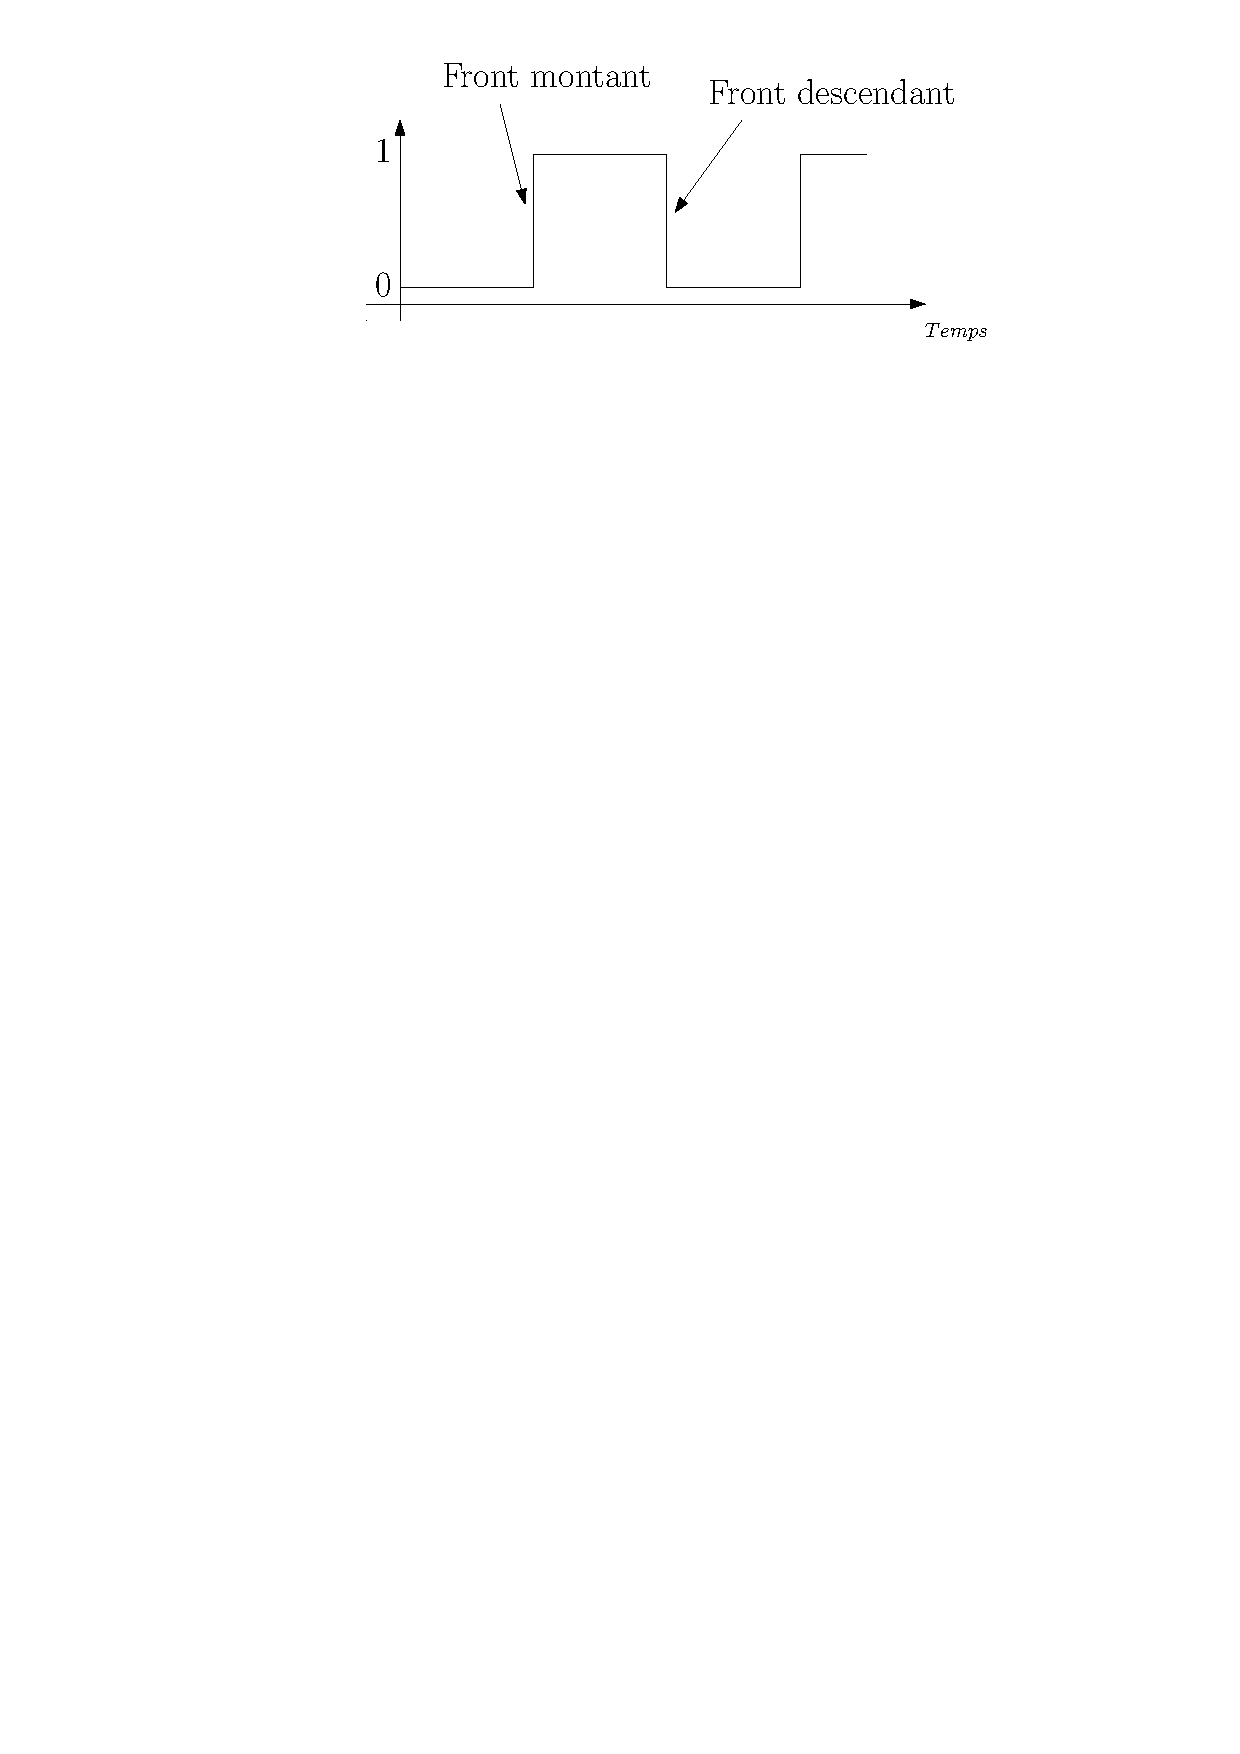
\includegraphics[width=0.5\linewidth]{Figs/clk_fronts.pdf}
\caption{\label{fig:clk_fronts} Le front montant d'un signal créneau est lorsque ce signal passe du niveau bas $0$ au niveau haut $1$. Le front descendant est lorsque le signal passe du niveau haut au niveau bas.}
\end{figure}

\subsection{Bascule D synchrone sur front montant : maître esclave}

En chaînant deux verrous D, on peut construire une mémoire mise à jour sur le front montant d'un signal d'horloge comme illustré sur la figure \ref{fig:flipflop_d}.

\begin{figure}[htbp]
   \begin{minipage}[c]{.7\linewidth}
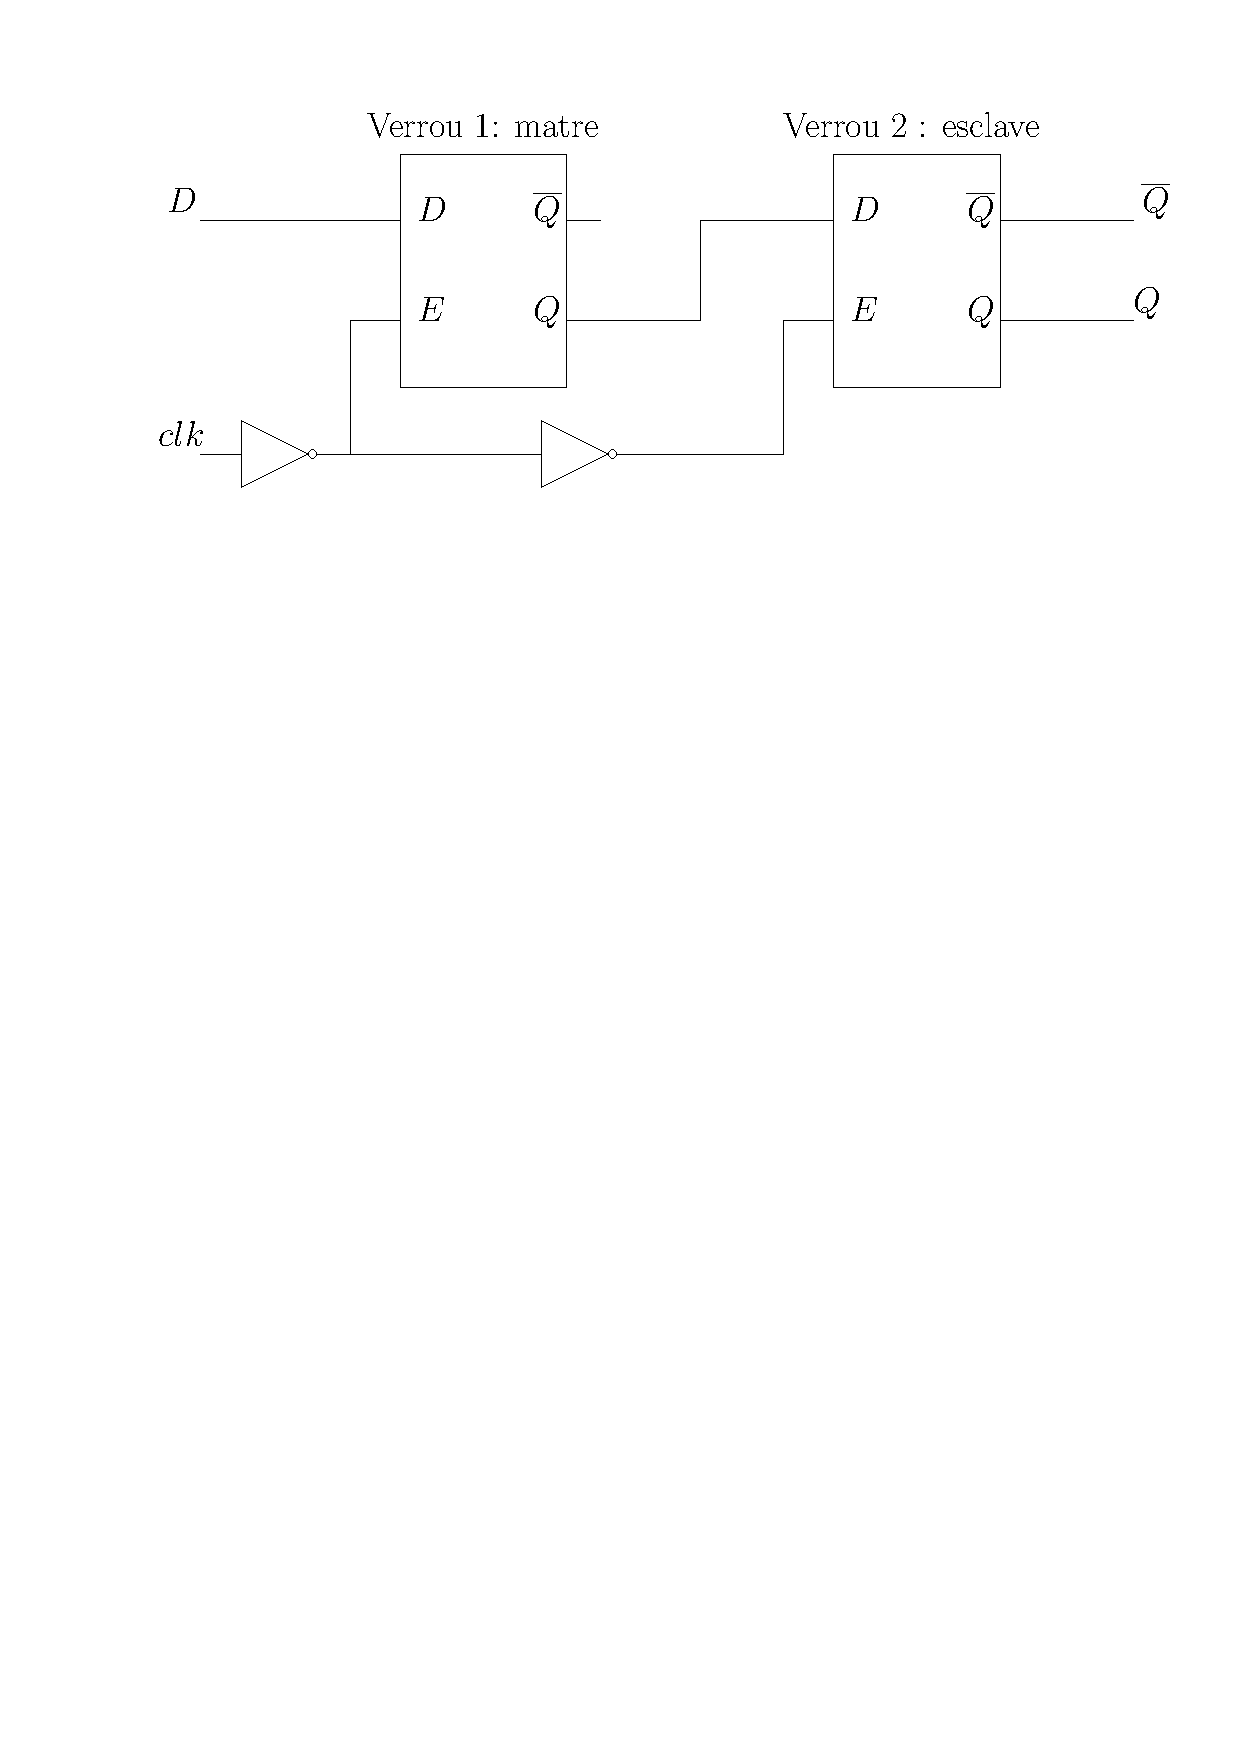
\includegraphics[width=\columnwidth]{Figs/flipflop_D.pdf}\\\centering a)
\end{minipage}\hfill
\begin{minipage}[c]{.2\linewidth}
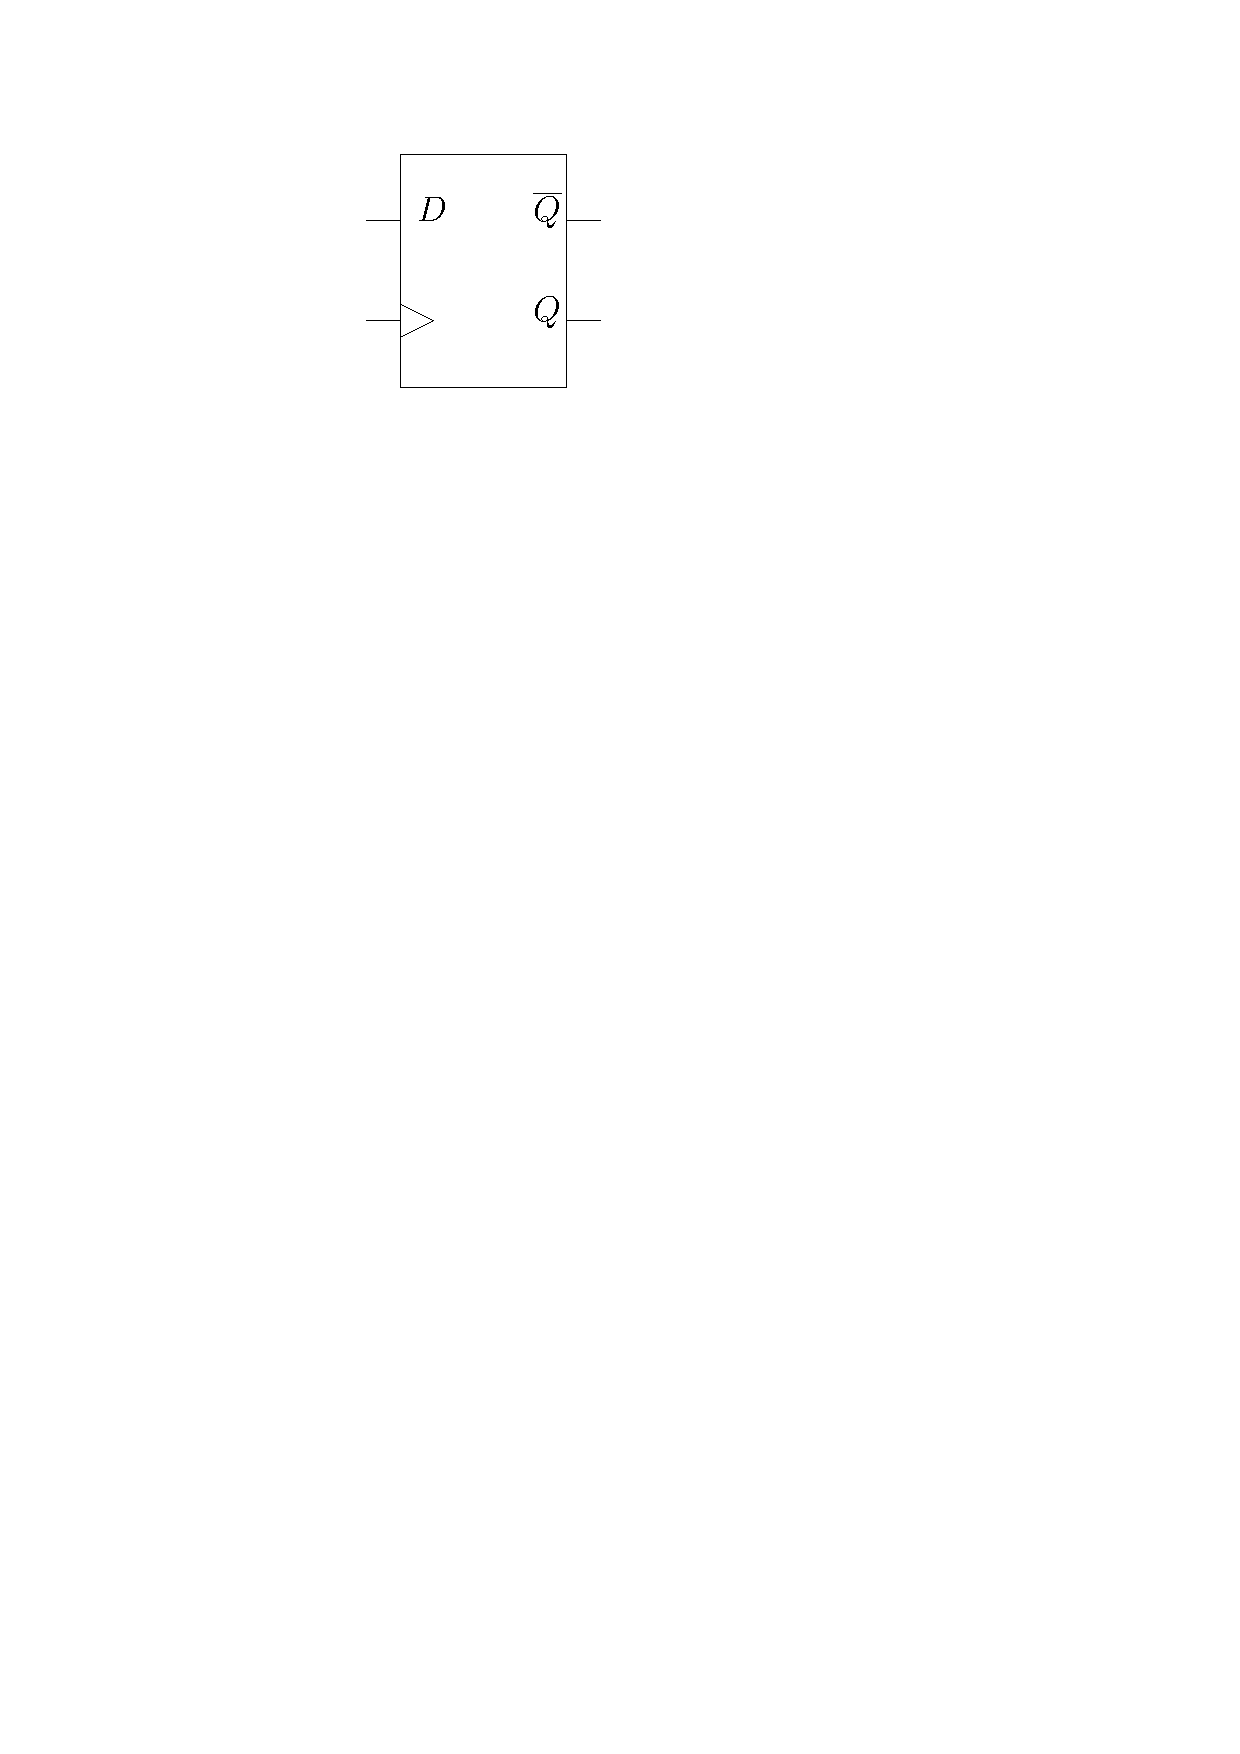
\includegraphics[width=\columnwidth]{Figs/flipflop_D_schema.pdf}
\\\centering b)
\end{minipage}
\caption{\label{fig:flipflop_d} a) Une bascule D (\emph{Data-flipflop}) construite à partir de deux verrous D respectivement appelés maître et esclave, dont la mise à jour n'est permise que sur un front montant d'horloge. b) Représentation schématique d'une bascule D. Le symbole en triangle indique un composant sensible au front montant d'horloge. Si il avait été sensible au front descendant, on aurait ajouté un petit cercle devant le triangle, à l'extérieur du composant (comme sur les portes inverseur).}
\end{figure}

Reprenons les entrées (D et Horloge) de la figure \ref{fig:chrono_verrou_D} et traçons le chronogramme des sorties des deux verrous sur la figure \ref{fig:chrono_flipflop_d}. Sur ce chronogramme, les entrées et sorties des deux verrous sont suffixés du numéro du verrou : $D_1$,$E_1$, $Q_1$ pour le premier verrou, le verrou maître et $D_2$, $E_2$ et $Q_2$ pour le second verrou, le verrou escale. Pour comprendre le fonctionnement de ce circuit, il suffit de considérer chacun des verrous l'un après l'autre en commençant par identifier quand les signaux Enable de chacun des verrous est à l'état haut et en recopiant l'entrée dans ce cas. Lorsque le signal Enable est à l'état bas, le verrou est dans l'état mémoire. Au final, si on ne se concentre que sur les entrées $D$, $Horloge$ et la sortie $Q = Q_2$, on constate que la sortie est une copie de l'entrée aux fronts montants de l'horloge, nous avons donc construit un circuit mémoire mis à jour sur les fronts montants de l'horloge (\emph{edge-triggered flip flop}).

\begin{figure}[htbp]
\begin{center}
\begin{tikztimingtable}[
    timing/coldist=2pt,     % column distance
    xscale=1,yscale=2, % scale diagrams
    semithick               % set line width
]
$Horloge$ & 8L 8H 8L 8H \\
$D=D_1$       & 2L 3H 2L 2H  1L 2H 1L 1H 1L 3H  6L   2L 3H 3L \\
$E_1$     & 8H 8L 8H 8L\\
$Q_1=D_2$     & 2L 3H 2L 1H 8H 2H 6L 8L\\
$E_2$     & 8L 8H 8L 8H\\
$Q=Q_2$       & 8L 8H 8H 8L\\
\extracode
  %\tablerules
  %\tablegrid
\end{tikztimingtable}
\end{center}
\caption{\label{fig:chrono_flipflop_d} Chronogramme d'une bascule D maître-escale sensible à un front montant d'horloge. La sortie de la bascule est la valeur de l'entrée $D$ au dernier front montant d'horloge.}
\end{figure}

Nous n'étudierons pas plus en détails le fonctionnement de la bascule D, sachez simplement qu'en pratique, le bon fonctionnement de la bascule est garantie si l'entrée est stable autour du front montant d'horloge, encadré par des temps de mise en place (\emph{setup time}) et de maintien (\emph{hold time}).

\subsection{Réalisation d'un verrou D avec un mutliplexeur}
\label{subsec:verrouD_multiplexeur}

Une autre réalisation possible d'un verrou peut se construire à partir d'un multiplexeur 2-1. Je vous rappelle qu'un multiplexeur à 2 entrées, un bit de sélection et une sortie peut être vu comme un aiguillage. Pour réaliser un verrou D avec un multiplexeur, il suffit de reboucler la sortie du multiplexeur sur la première entrée de telle sorte que si le bit de sélection vaut $0$, le circuit soit dans un état mémoire et de présenter l'entrée $D$ comme deuxième entrée du multiplexeur de telle sorte que le circuit soit transparent lorsque le bit de sélection vaut $1$. Il faudra néanmoins faire attention à utiliser la réalisation du multiplexeur sans aléas statiques. En effet, avec le multiplexeur ayant un aléa statique, si $S=1$, $D=1$ et $Q=1$, lorsque le multiplexeur est basculé dans l'état mémoire $S=1 \rightarrow S=0$, l'aléa de sortie conduit à oublier $Q=1$ et à mémoriser $Q=0$.

\subsection{Registre et mémoire RAM (Random Access Memory)}

\subsubsection{Registre à $n$ bits sur front montant}

La bascule D (maître-escale par exemple) permet de mémoriser un bit d'information et est mise à jour sur un front montant d'horloge. Pour pouvoir mémoriser un mot de plus de $n$ bits, il suffit de considérer $n$ bascules D et de construire ce qu'on appelle \textbf{un registre à n bits}, représenté sur la figure \ref{fig:registre}. Les entrées $Enable$ et $Clear$ apparaissent parfois. L'entrée $Enable$ permet d'autoriser le registre à se mettre à jour. Si l'entrée Enable est à $0$, aucune mise à jour du contenu du registre n'aura lieu. L'entrée Clear permet de remettre à $0$ le contenu du registre $Q=000\cdots$ de manière asynchrone, i.e. sans attendre de front montant d'horloge.

\begin{figure}[htbp]
   \begin{minipage}[c]{.2\linewidth}
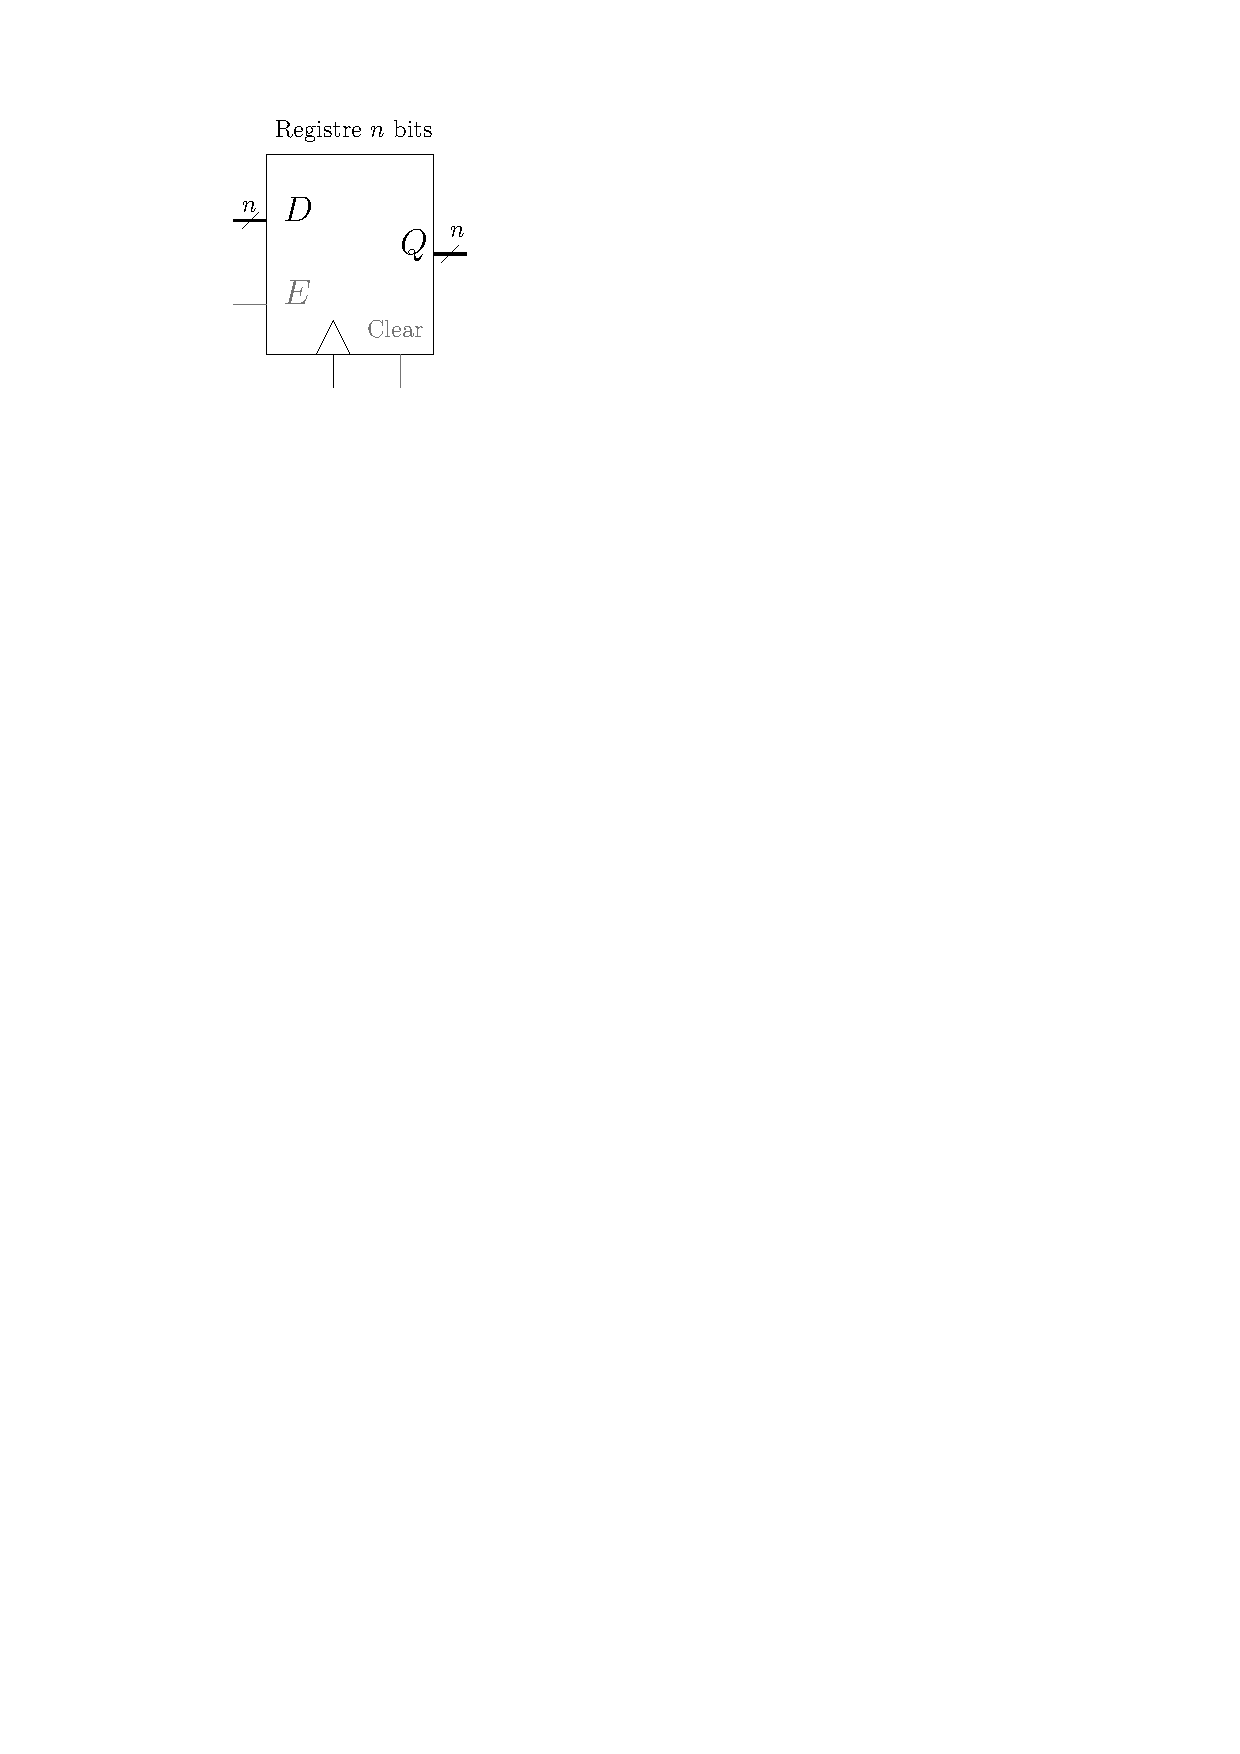
\includegraphics[width=\columnwidth]{Figs/registre.pdf}\\\centering a)
\end{minipage}\hfill
\begin{minipage}[c]{.4\linewidth}
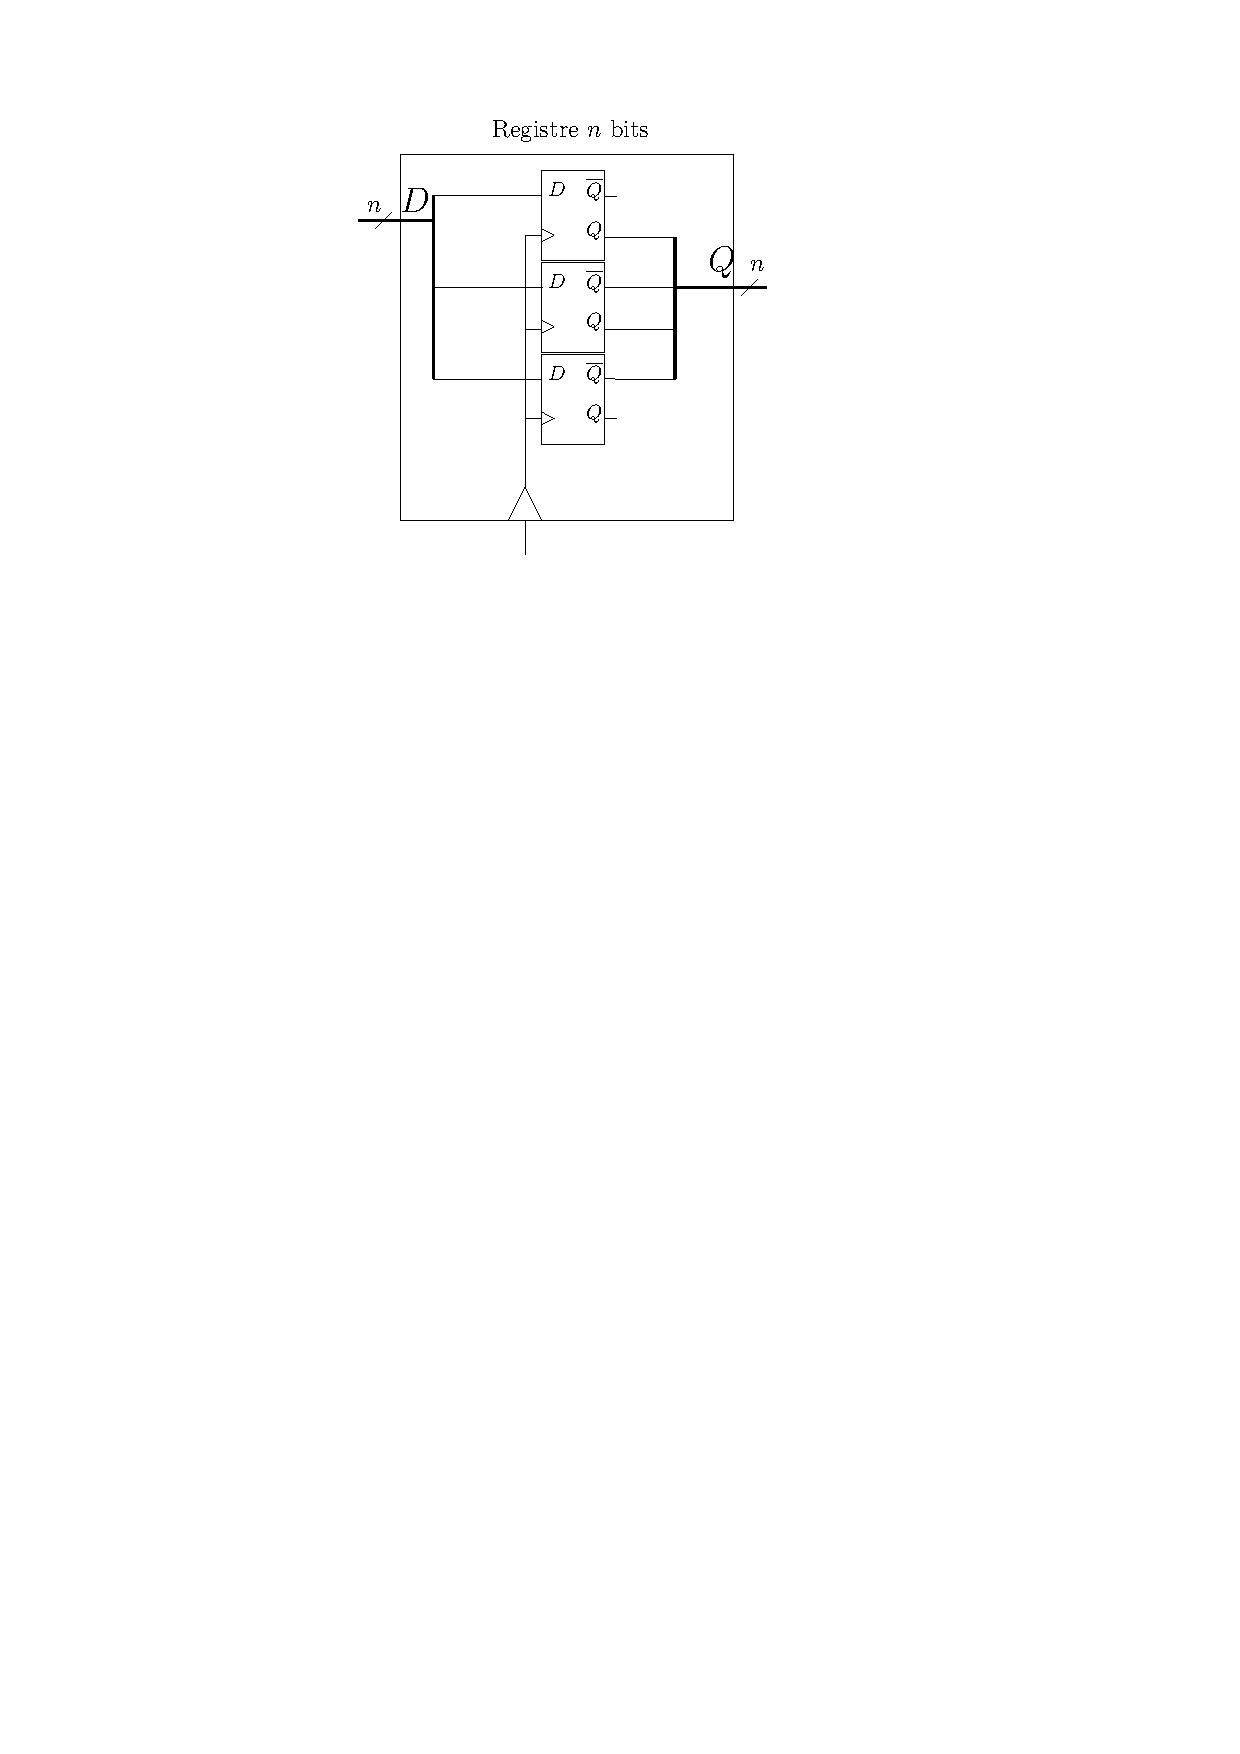
\includegraphics[width=\columnwidth]{Figs/registre_inner.pdf}
\\\centering b)
\end{minipage}
\caption{\label{fig:registre} a) Un registre actif sur front montant à $n$ bits. Les entrées $E$ et $Clear$ sont parfois disponibles. L'entrée $E$ autorise la mise à jour du registre et doit être au niveau haut pour que les signaux d'horloge soient opérants. L'entrée Clear permet de remettre à $0$ de manière asynchrone le contenu du registre. b) Un registre à $n$ bits sur front montant peut se construire à l'aide de $n$ bascules D sur front montant.}
\end{figure}


\subsubsection{Mémoire en lecture et écriture (RAM)}

Au même titre que combiner $n$ bascules $D$ permet de mémoriser un mot de $n$ bits, on peut aussi combiner $2^k$ registres pour mémoriser $2^k$ mots de $n$ bits comme sur la figure \ref{fig:ram}. Pour l'écriture, l'activation de l'un ou l'autre des registres se fait par l'entrée $Enable$ alimentées par la sortie d'un décodeur. Pour la lecture, le registre sélectionné par l'adresse est dirigé en sortie grâce à un multiplexeur. On dispose alors d'un contenu dit adressable. En effet l'entrée $Adr$ de $k$ bits permet de sélectionner l'un ou l'autre des $2^k$ registres soit en écriture, soit en lecture. Le choix entre l'écriture et la lecture se fait par des entrées supplémentaires Load et Store (parfois combinées en une seule).

\begin{figure}[htbp]
   \begin{minipage}[c]{.4\linewidth}
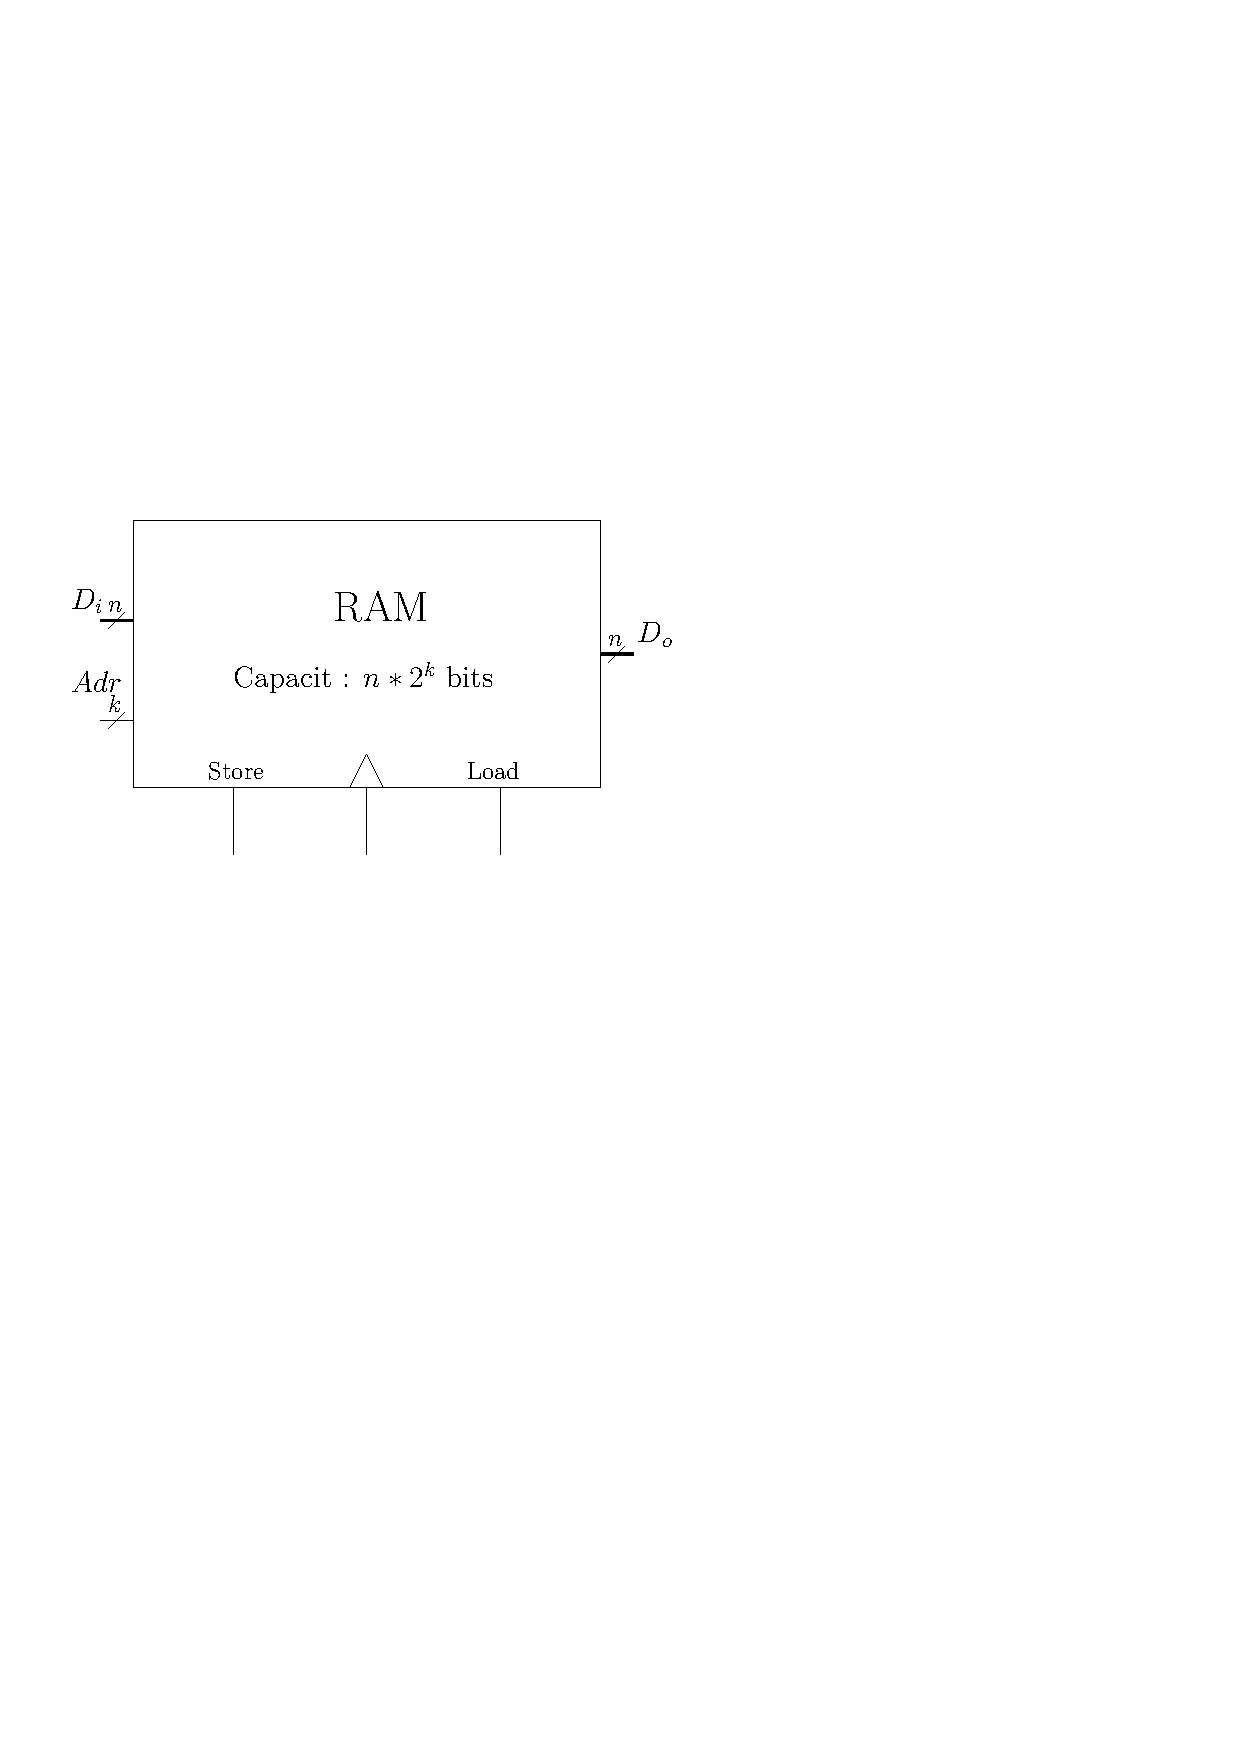
\includegraphics[width=\columnwidth]{Figs/ram.pdf}\\\centering a)
\end{minipage}\hfill
\begin{minipage}[c]{.4\linewidth}
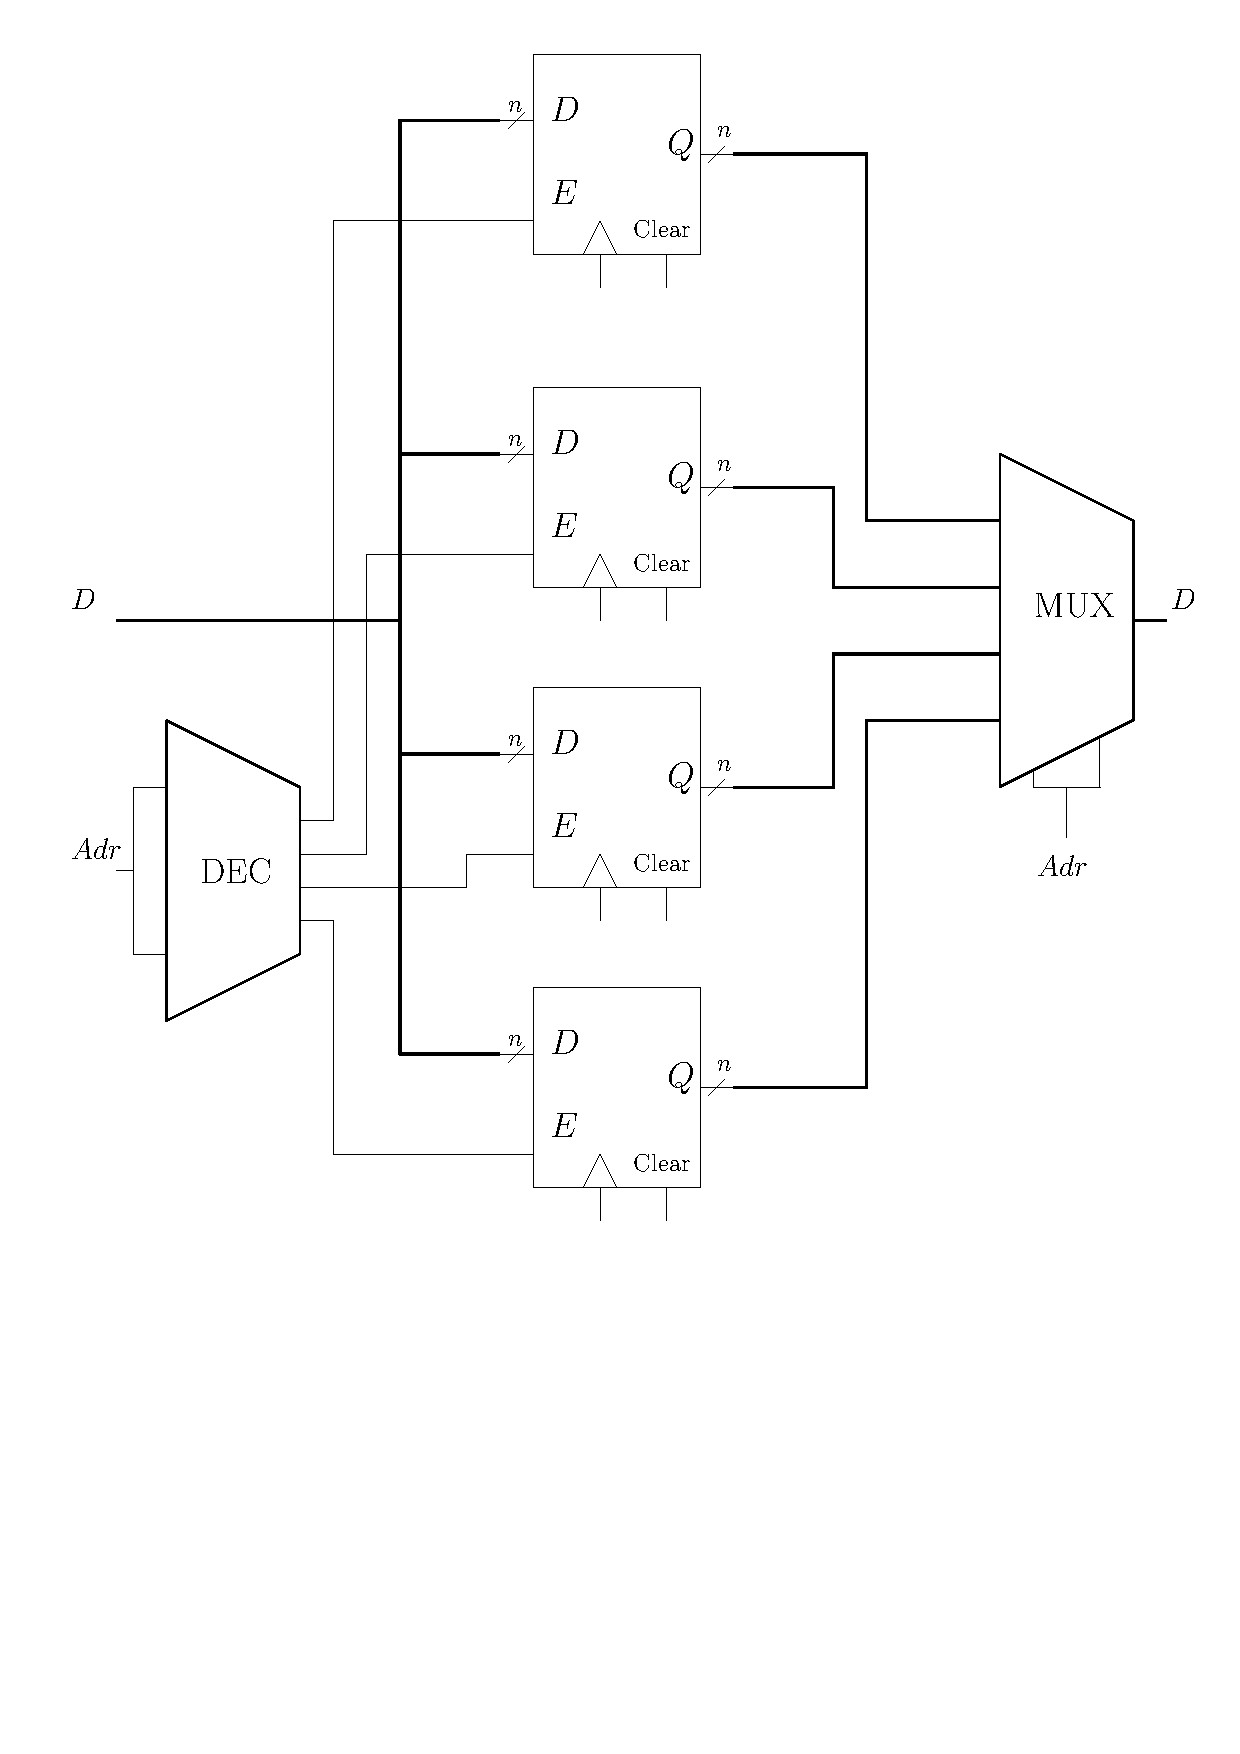
\includegraphics[width=\columnwidth]{Figs/ram_inner.pdf}
\\\centering b)
\end{minipage}
\caption{\label{fig:ram} a) Illustration schématique d'une RAM de capacité $n 2^k$ disposant d'une entrée $D_i$ et d'une sortie $D_o$ sur $n$ bits : l'une pour le stockage l'autre pour le chargement, d'une ligne d'adresse sur $k$ bits, d'un signal d'horloge, et de signaux de contrôle pour autoriser le chargement ou le stockage de données. b) Une partie de l'organisation interne d'une RAM. Il manque sur ce schéma le circuit permettant de piloter le chargement (load) et le stockage (store) des données. }
\end{figure}

On distingue deux opérations avec les mémoires RAM : le chargement (load) et le stockage (store). Le chargement vise à placer sur le bus de données de sortie $D$, la valeur du contenu du registre adressé par l'entrée $Adr$. Le stockage vise à modifier le contenu du registre adressé par l'entrée $Adr$ avec la valeur présente sur le bus d'entrée $D$. Pour charger une valeur sur le bus de sortie il faudra :
\begin{itemize}
\item placer sur le bus d'adresse l'adresse du mot à lire
\item le mot à l'adresse $Adr$ est directement accessible sur le bus de sortie
\end{itemize}

Pour stocker une nouvelle valeur dans la mémoire, il faudra :
\begin{itemize}
\item placer sur le bus d'adresse l'adresse du mot à écrire
\item placer sur le bus de données la valeur à stocker
\item déclencher un front montant d'horloge et la nouvelle valeur sera stockée en mémoire
\end{itemize}

On parle de mémoire RAM (\emph{Random Access Memory}) puisque le temps d'accès en lecture/écriture d'un mot à une adresse donnée est indépendant de l'adresse.


%\textbf{Illustration du rôle de la bascule D : le registre à décalage}\\
%\textbf{Illustration avec le compteur par incrément : 2 bascules D avec rebouclage}\\
